\documentclass[12pt, letterpaper]{article}

% --- Packages ---
\usepackage{geometry}
 \geometry{margin=1in}
\usepackage{graphicx}
\usepackage{amsmath, amssymb}
\usepackage{booktabs}
\usepackage{hyperref}
\usepackage{cite}
\usepackage{setspace}
\onehalfspacing
\usepackage{fontspec}
\usepackage{polyglossia}
\setmainlanguage{vietnamese}

% --- Metadata ---
\title{Cài đặt hệ điều hành mã nguồn mở Lubuntu 24.04 trên máy tính cầm tay}
\author{Đỗ Hoàng Gia Bảo - 23020783 \\ \small Khoa Điện tử - Viễn Thông}
\date{\today}

\begin{document}

\maketitle

\begin{abstract}
Báo cáo này trình bày quá trình tải phần mềm, cài đặt hệ điều hành mã nguồn mở Lubuntu 24.04 trên máy tính cầm tay. 
\end{abstract}

% --- Front Matter (Roman Numerals) ---
\newpage
\tableofcontents

% --- Main Content (Arabic Numerals) ---
\newpage
\pagenumbering{arabic}
\setcounter{page}{3} % This automatically resets the counter to 1

\section{Các bước tải phần mềm và cài đặt hệ điều hành}
\subsection{Tải phần mềm}
Truy cập vào trang web chính thức của Lubuntu tại \url{https://lubuntu.me/downloads/} và chọn phiên bản 24.04 để tải về.\\
Sau đó chọn phương thức tải file .iso phù hợp với máy tính cầm tay của bạn (thường là 64-bit).\\
Sau khi tải xong, trên máy sẽ có một file .iso chứa hệ điều hành Lubuntu 24.04.

\subsection{Cài đặt hệ điều hành}
Sử dụng phần mềm tạo USB bootable như Rufus hoặc Etcher để ghi file .iso vào một USB.\\
Khởi động lại máy tính cầm tay và vào BIOS/UEFI để thiết lập khởi động từ USB.\\
Làm theo hướng dẫn trên màn hình để cài đặt Lubuntu 24.04 lên máy tính cầm tay.\\
Chọn phân vùng cài đặt (dual boot hoặc xóa ổ nhớ) và hoàn tất quá trình cài đặt.\\
Sau khi cài đặt xong, khởi động lại máy và đăng nhập vào hệ điều hành mới cài đặt.

\section{Kết quả và đánh giá}
Sau khi cài đặt thành công, máy tính cầm tay đã chạy Lubuntu 24.04 một cách ổn định.

\begin{figure}[ht]
    \centering
    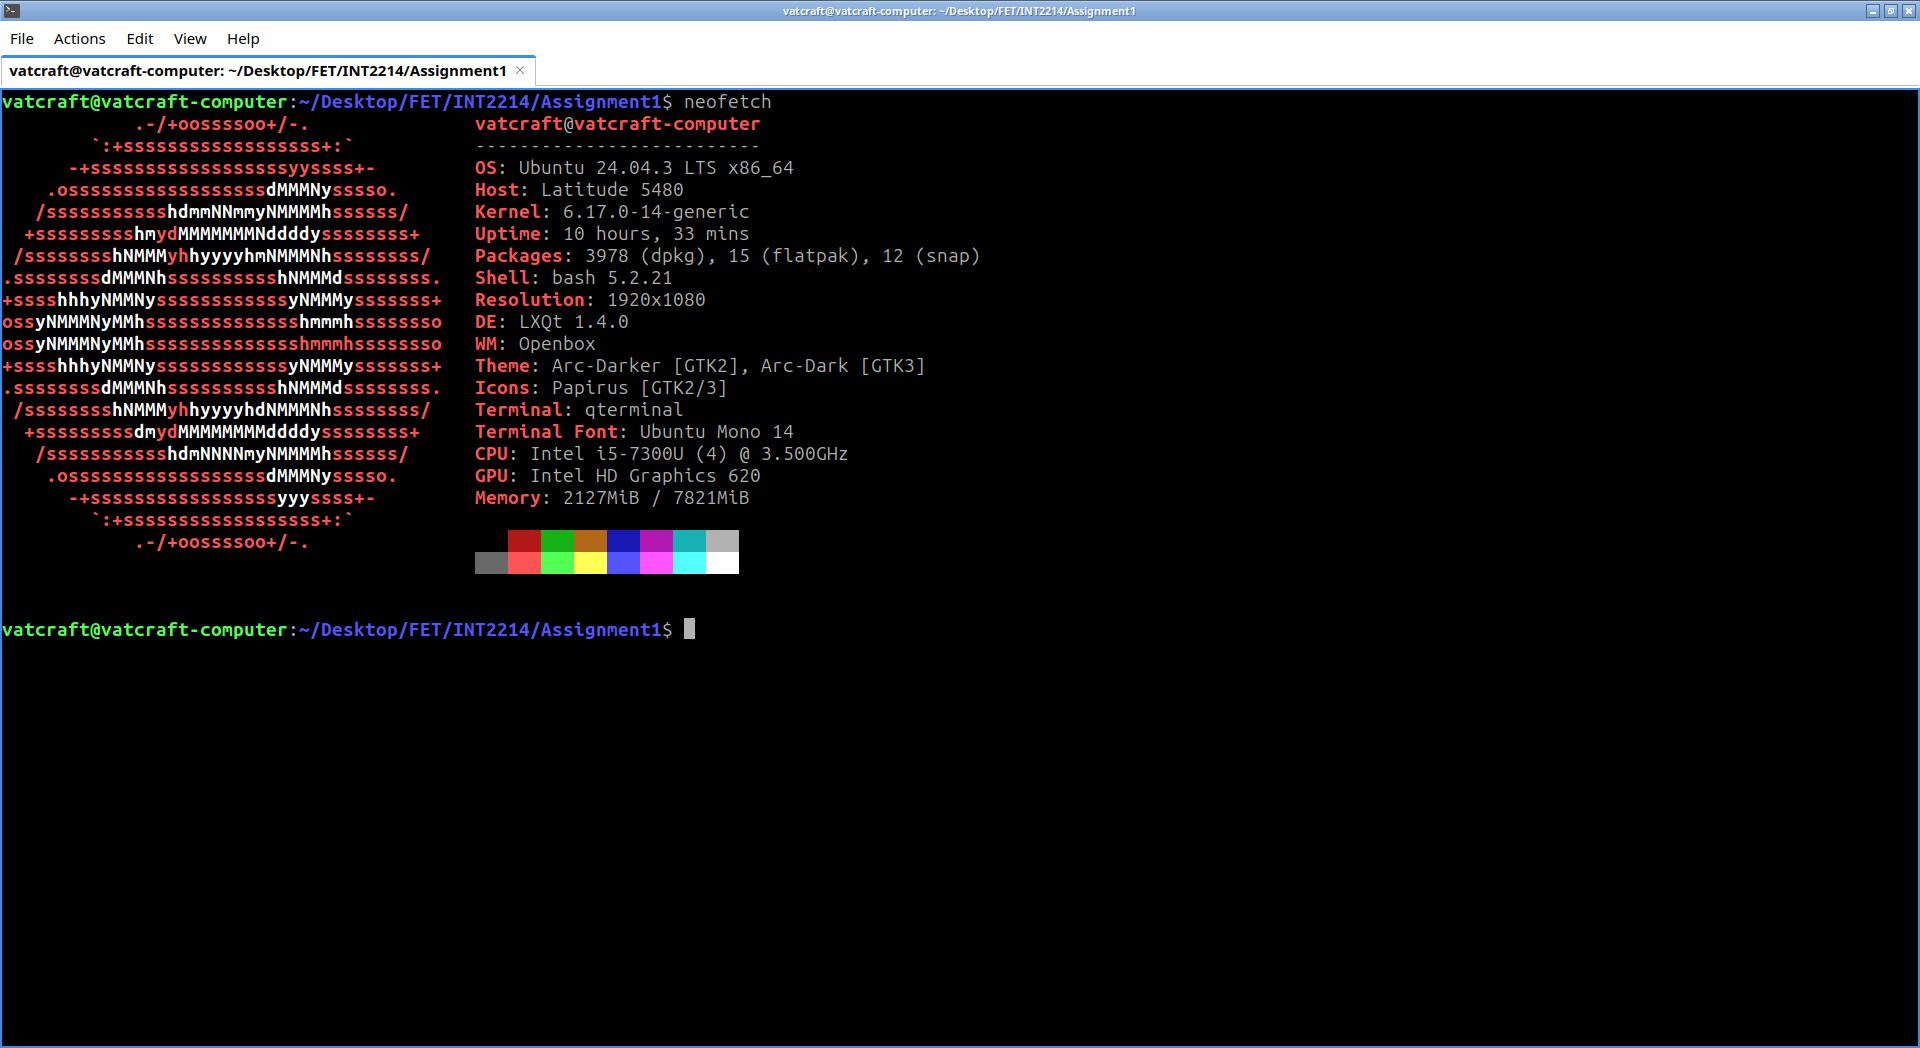
\includegraphics[width=0.8\textwidth]{screen.jpg}
    \caption{Terminal xác nhận Lubuntu 24.04 đã được cài đặt thành công.}
    \label{fig:terminal}
\end{figure}

\end{document}